\documentclass[12pt]{article}
\usepackage{geometry}
 \geometry{
 letterpaper,
 left=2.54cm,
 right=2.54cm,
 bottom=2.54cm,
 top=2.54cm,
 }
\usepackage[utf8]{inputenc}

%% appendix
\usepackage{appendix}
%% biblatex
\usepackage[style=apa,language=american,maxnames=4,minnames=3,sortcites=true]{biblatex}
\DeclareLanguageMapping{american}{american-apa}
\addbibresource{ref.bib}
%% uses times font
\usepackage{mathptmx}
%% set fontsize
\fontsize{12}{1} \selectfont
%% set line spacing
\usepackage{setspace}
\singlespacing
%% set par indent
%\usepackage{indentfirst}
\setlength{\parindent}{6.5ex}
%% customize heading styles
\usepackage[indentafter]{titlesec}
%%%% heading 1
\titleformat{\section}
  {\normalsize\center}
  {}
  {0pt}
  {\MakeUppercase}
%%%% heading 2
\titleformat{\subsection}
  {\normalsize\center\bf}
  {}
  {0pt}
  {\capitalize}
%%%% heading 3
\titleformat{\subsubsection}
  {\normalsize\bf}
  {}
  {0pt}
  {\capitalize}
%\titleformat{⟨command⟩}[⟨shape⟩]{⟨format⟩}{⟨label⟩}{⟨sep⟩}{⟨before-code⟩}[⟨after-code⟩]

%%%%%% start: define some macros here %%%%%%
\newcommand{\longvertspacing}{~\\~\\~\\~\\~\\~\\}
\newcommand{\mylinespacing}{\vspace{1em}}
\newcommand{\myoptpg}{\textbf{THIS PAGE IS OPTIONAL}}
\newcommand{\mytitle}{my dissertation title}
\newcommand{\myname}{Zhiya Zuo}
\newcommand{\mydegree}{DEGREE NAME}
\newcommand{\myprogram}{PROGRAM NAME}
\newcommand{\mymonth}{May}
\newcommand{\myyear}{2019}
\newcommand{\myadvisor}{Associate Professor Kang Zhao}
%% a new center environment
\newenvironment{tightcenter}{%
  \setlength\topsep{0pt}
  \setlength\parskip{0pt}
  \begin{center}
}{%
  \end{center}
}
%% adjust quotation environment margin
\renewenvironment{quote}{%
   \list{}{%
     \leftmargin0cm   % this is the adjusting screw
     \rightmargin\leftmargin
   }
   \item\relax
}
{\endlist}
%%%%%% end: define some macros here %%%%%%

%%%%%% capitalize from stackexchange %%%%%% 
\usepackage{ifxetex}

\usepackage{xparse}

\ExplSyntaxOn
\NewDocumentCommand{\capitalize}{>{\SplitList{~}}m}
 {
  \seq_clear:N \l_capitalize_words_seq
  \ProcessList{#1}{\CapitalizeFirst}
  \seq_use:Nn \l_capitalize_words_seq { ~ }
 }
\NewDocumentCommand{\CapitalizeFirst}{m}
 {
  \capitalize_word:n { #1 }
 }

\sys_if_engine_pdftex:TF
 {
  \cs_set_eq:Nc \capitalize_tl_set:Nn { protected@edef }
 }
 {
  \cs_set_eq:NN \capitalize_tl_set:Nn \tl_set:Nn
 }

\cs_new_protected:Nn \capitalize_word:n
 {
  \capitalize_tl_set:Nn \l_capitalize_word_tl { #1 }
  \seq_if_in:NfTF \g_capitalize_exceptions_seq { \tl_to_str:n { #1 } }
   % exception word
   { \seq_put_right:Nn \l_capitalize_words_seq { #1 } } % exception word
   % to be uppercased
   { \seq_put_right:Nx \l_capitalize_words_seq { \tl_mixed_case:V \l_capitalize_word_tl } }
 }
\cs_generate_variant:Nn \tl_mixed_case:n { V }
\NewDocumentCommand{\AppendToList}{m}
 {
  \clist_map_inline:nn { #1 }
   {
    \seq_gput_right:Nx \g_capitalize_exceptions_seq { \tl_to_str:n { ##1 } }
   }
 }
\cs_generate_variant:Nn \seq_if_in:NnTF { Nf }
\seq_new:N \l_capitalize_words_seq
\seq_new:N \g_capitalize_exceptions_seq
\ExplSyntaxOff

\AppendToList{a,is,of,óf}
%%%%%% capitalize from stackexchange %%%%%% 

\title{\MakeUppercase{\normalsize\mytitle}\vspace{-2em}}
\author{\vspace{-5ex}}
\date{\vspace{-5ex}}

\begin{document}

\maketitle
\longvertspacing
\begin{tightcenter}
    by
\end{tightcenter}
\mylinespacing
\begin{tightcenter}
    \myname
\end{tightcenter}
\longvertspacing
\begin{tightcenter}
A thesis submitted in partial fulfillment \\
of the requirements for the \\
\mydegree~\\
degree in \myprogram~in the  \\
Graduate College of \\
The University of Iowa
\end{tightcenter}
\mylinespacing
\begin{tightcenter}
\mymonth~\myyear
\end{tightcenter}
\mylinespacing
\begin{tightcenter}
Thesis Supervisor: \myadvisor
\end{tightcenter}

%% copyright page %%
\pagenumbering{gobble} 
\vspace*{\fill} 
\begin{quote} 
\centering 
Copyright by\\ 
\mylinespacing
\myname \\
\mylinespacing
\myyear \\
\mylinespacing
All rights reserved \\
\mylinespacing
\myoptpg
\end{quote}
\vspace*{\fill}

%% copyright page %%

%% dedication page %%
\vspace*{\fill} 
\noindent
To (Prior to your first thesis deposit, delete this text and type your dedication here.  The entire dedication should be single spaced and centered vertically and horizontally on the page.  This text may be altered between first and final deposit.)
\begin{quote}
\centering
\mylinespacing
\myoptpg
\end{quote}
\vspace*{\fill}
%% dedication page %%

%% epigraph page %%
\vspace*{\fill} 
\begin{quote}
\centering
Prior to thesis deposit, delete this text and type your epigraph here.  Each line should be centered, single spaced, and the entire text centered vertically.  This text may be altered between first and final deposits.\\
\mylinespacing
\myname \\
\mytitle \\
\mylinespacing
\myoptpg
\end{quote}
\vspace*{\fill}
%% epigraph page %%

%% ack page %%
\begin{doublespace}
\begin{tightcenter}
ACKNOWLEDGEMENTS
\mylinespacing
\end{tightcenter}

Prior to your first thesis deposit, replace this text with your acknowledgements.  This text should be double spaced and each paragraph should be indented.  This text may be altered between first and final deposit.

Prior to your first thesis deposit, replace this text with your acknowledgements.  This text should be double spaced and each paragraph should be indented.  This text may be altered between first and final deposit.  
\mylinespacing
\begin{tightcenter}
\myoptpg
\end{tightcenter}
\end{doublespace}

%% ack page %%

%% abs page %%
\begin{doublespace}
\begin{tightcenter}
ABSTRACT
\mylinespacing
\end{tightcenter}

Prior to your first thesis deposit, replace this text with the text of your scientific/ scholarly abstract. The text of this abstract should be double spaced and each new paragraph should be indented. This text may be altered between first and final deposits.

\mylinespacing
\mylinespacing
\begin{tightcenter}
\textbf{This abstract is required for everyone except DMA and MFA students.}
\end{tightcenter}
\end{doublespace}

%% abs page %%

%% public abs page %%
\begin{doublespace}
\begin{tightcenter}
PUBLIC ABSTRACT
\mylinespacing
\end{tightcenter}

Prior to your first thesis deposit, replace this text with the text of your public abstract. The text of this abstract should be double spaced and each new paragraph should be indented. The text may be altered between first and final deposits. This abstract is required for all thesis/dissertations. 

The public abstract is to be placed at this point in your first and final deposit and submitted via webform at final deposit. This abstract may be up to 250 words and should be written for a non-academic lay audience. In writing your public abstract, avoid jargon and technical language as much as possible. 

The ability to communicate research simply and clearly is an important skill when interviewing for faculty positions, as well as for positions in industry and alt-ac sectors. The public abstract helps convey ideas beyond one’s immediate academic circle, facilitating communication with colleagues who do different kinds of work and possess different dimensions of training.

Think of your public abstract as your “elevator pitch” or what you might tell someone who asks, “What is your thesis about?” You may only have a few minutes to explain it to them while keeping their attention and using terminology you are sure they will understand without further lengthy explanation.

Another way to think of your public abstract is like the description you would read on the inside of a book cover.

\end{doublespace}

%% public abs page %%

%% content lists %%
\setcounter{tocdepth}{2} % can change 2 for deeper levels
\tableofcontents
\newpage
\listoftables
\newpage
\listoffigures

%% content lists %%

%% preface %%
\begin{doublespace}
\begin{tightcenter}
PREFACE
\mylinespacing
\end{tightcenter}

Prior to your first deposit, replace this text with the text of your Preface. The Preface should be double spaced and new paragraphs should be indented. This text may be altered between first and final deposits.

\mylinespacing
\mylinespacing
\begin{tightcenter}
\myoptpg
\end{tightcenter}
\end{doublespace}
%% preface %%

\begin{doublespace}
%% main contents %%

\section{heading 1: test ttest testtest testest test}

Lorem ipsum dolor sit amet, consectetuer adipiscing elit.  Ut purus elit, vestibulum ut, placeratac,  adipiscing vitae,  felis.   Curabitur dictum gravida mauris.  

Nam arcu libero,  nonummy eget,consectetuer id, vulputate a, magna. Donec vehicula augue eu neque. Pellentesque habitant morbitristique senectus et netus et malesuada fames ac turpis egestas. Mauris ut leo. Cras viverra metusrhoncus sem.  Nulla et lectus vestibulum urna fringilla ultrices. 

I want to cite something here \parencite{zuo2019standing}. I want to want to try cite~\textcite{zuo2019standing} with in-line style.

\subsection{heading 2: use for your broadest subheading level, centered, bold, uppercase and lowercase}

Lorem ipsum dolor sit amet, consectetuer adipiscing elit.  Ut purus elit, vestibulum ut, placeratac,  adipiscing vitae,  felis.   Curabitur dictum gravida mauris. 

\subsubsection{heading 3: use for your next heading level, left-aligned, bold, uppercase and lowercase}

Lorem ipsum dolor sit amet, consectetuer adipiscing elit. 

%% main contents %%

%% ref %%
\printbibliography
%% ref %%

%% appendix %%
\appendix
\newcommand{\hbAppendixPrefix}{A}
\renewcommand{\thefigure}{\hbAppendixPrefix.\arabic{figure}}
\setcounter{figure}{0}
\renewcommand{\thetable}{\hbAppendixPrefix.\arabic{table}} 
\setcounter{table}{0}

\section{APPENDIX \hbAppendixPrefix: Test for appendix}

Lorem ipsum dolor sit amet, consectetuer adipiscing elit.  Ut purus elit, vestibulum ut, placeratac,  adipiscing vitae,  felis.   Curabitur dictum gravida mauris.  
\renewcommand{\hbAppendixPrefix}{B}
\renewcommand{\thefigure}{\hbAppendixPrefix.\arabic{figure}}
\setcounter{figure}{0}
\renewcommand{\thetable}{\hbAppendixPrefix.\arabic{table}} 
\setcounter{table}{0}

\section{APPENDIX \hbAppendixPrefix: Test for another appendix}

Lorem ipsum dolor sit amet, consectetuer adipiscing elit.  Ut purus elit, vestibulum ut, placeratac,  adipiscing vitae,  felis.   Curabitur dictum gravida mauris.
Let me add a figure here~\cref{fig:chap_1}:

\begin{center}
    \bxfigure[!hb]{Some figure\label{fig:chap_1}}{
    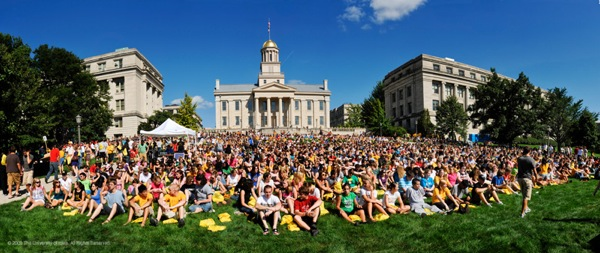
\includegraphics[width=0.9\columnwidth]{fig1}
}
\end{center}

%% appendix %%


\end{doublespace}


\end{document}
